%
% IEEE Transactions on Microwave Theory and Techniques example
% Tibault Reveyrand - http://www.microwave.fr
%
% http://www.microwave.fr/LaTeX.html
% ---------------------------------------



% ================================================
% Please HIGHLIGHT the new inputs such like this :
% Text :
%  \hl{comment}
% Aligned Eq.
% \begin{shaded}
% \end{shaded}
% ================================================



\documentclass[journal]{IEEEtran}

%\usepackage[retainorgcmds]{IEEEtrantools}
%\usepackage{bibentry}
\usepackage{xcolor,soul,framed} %,caption

\colorlet{shadecolor}{yellow}
% \usepackage{color,soul}
\usepackage[pdftex]{graphicx}
\graphicspath{{../pdf/}{../jpeg/}}
\DeclareGraphicsExtensions{.pdf,.jpeg,.png}

\usepackage[cmex10]{amsmath}
%Mathabx do not work on ScribTex => Removed
%\usepackage{mathabx}
\usepackage{array}
\usepackage{mdwmath}
\usepackage{mdwtab}
\usepackage{eqparbox}
\usepackage{url}


% ----------------------------------------------

% Definitions of languages: ------------
\usepackage{listings}
\lstdefinestyle{cStyle}{
  basicstyle=\scriptsize,
  breakatwhitespace=false,
  breaklines=true,
  captionpos=b,
  keepspaces=true,
  numbersep=5pt,
  showspaces=false,
  gobble=4,
  tabsize=4,
  showstringspaces=false,
  showtabs=false,
}
\renewcommand*{\lstlistingname}{Code}

% ----------------------------------------------




\hyphenation{op-tical net-works semi-conduc-tor}

%\bstctlcite{IEEE:BSTcontrol}


%=== TITLE & AUTHORS ====================================================================
\begin{document}
\bstctlcite{IEEEexample:BSTcontrol}
    \title{Otimizations Based on Population Methods}
  \author{Carlos~Matheus~Barros~da~Silva,~\IEEEmembership{Bachelor Student of ITA}\\Prof. Marcos~Ricardo~Omena~de~Albuquerque~Máximo}


% The paper headers
\markboth{INSTITUTO TECNOLÓGICO DE AERONÁUTICA, APRIL~2019
}{Otimizations Based on Population Methods}


% ====================================================================
\maketitle



% === ABSTRACT ==============================================================
% ============================================================================
\begin{abstract}
%\boldmath
In this paper is avaliated a population based optimization called Particle Swarm Optimization (PSO). In order evaluate it, it was tested on a test functon, and on a control problem - optimization of proportional–integral–derivative controller parameters. It was seen that \textit{PSO} can find fast a solution, although it can get easily stocked on a local maximum. Its soluitons however are usualy good enought for a number of problems.
\end{abstract}


% === KEYWORDS ===============================================================
% ============================================================================
\begin{IEEEkeywords}
    Particle Swarm Optimization, PSO, population based optimization, optimization, proportional–integral–derivative controller, PID
\end{IEEEkeywords}






% For peer review papers, you can put extra information on the cover
% page as needed:
% \ifCLASSOPTIONpeerreview
% \begin{center} \bfseries EDICS Category: 3-BBND \end{center}
% \fi
%
% For peerreview papers, this IEEEtran command inserts a page break and
% creates the second title. It will be ignored for other modes.
\IEEEpeerreviewmaketitle


% ====================================================================
% ====================================================================
% ====================================================================


% === I. INTRODUCTION ========================================================
% =============================================================================
\section{Introduction}

\IEEEPARstart{I}{n} computer science, particle cloud optimization or particle swarm optimization (known by its acronym in English: PSO, of particle swarm optimization) refers to a metaheuristic that evokes the behavior of particles in nature.

PSO allows to optimize a problem from a population of candidate solutions, denoted as "particles", moving them throughout the search space according to mathematical rules that take into account the position and velocity of the particles. The movement of each particle is influenced by its best local position found so far, as well as by the best global positions found by other particles as they travel through the search space. The theoretical foundation of this is to make the particle cloud converge rapidly towards the best solutions.

PSO is a metaheuristic, since it assumes few or no hypotheses about the problem to be optimized and can be applied in large spaces of candidate solutions. However, like all metaheuristics, PSO does not guarantee obtaining an optimal solution in all cases.


% === II. Harmonically-Terminated Power Rectifier Analysis =================
% ==========================================================================
\section{Particle Swarm Optimization (PSO) Implementation}

The implementation was based on the file \textit{particle swarm optimization}. The essence is on \textit{ParticleSwarmOptimization} Class and \textit{Particle} Class development. The first one provides the interface in which the simulation communicates with the PSO.

Based on this, the development of \textit{ParticleSwarmOptimization} Class was oriented on receive inputs, provides information, and have methods that triggers the algorithm continuation.

In order to achieve this, it was developed the methods shown from the Code \ref{code:particle_swarm_optimization} to the Code \ref{code:notify_evaluation}.

\lstinputlisting[
    language=python,
    caption={Constructor of \textit{PSO} Class.},
    label={code:particle_swarm_optimization},
    style=cStyle,
    firstline=78,
    lastline=85
]{./../code/particle_swarm_optimization.py}

\lstinputlisting[
    language=python,
    caption={Method \textit{get best position} of \textit{PSO} Class.},
    label={code:get_best_position},
    style=cStyle,
    firstline=93,
    lastline=94
]{./../code/particle_swarm_optimization.py}

\lstinputlisting[
    language=python,
    caption={Method \textit{get best value} of \textit{PSO} Class.},
    label={code:get_best_value},
    style=cStyle,
    firstline=101,
    lastline=101
]{./../code/particle_swarm_optimization.py}

\lstinputlisting[
    language=python,
    caption={Method \textit{get position to evaluate} of \textit{PSO} Class.},
    label={code:get_position_to_evaluate},
    style=cStyle,
    firstline=110,
    lastline=111
]{./../code/particle_swarm_optimization.py}

\lstinputlisting[
    language=python,
    caption={Method \textit{advance generation} of \textit{PSO} Class.},
    label={code:advance_generation},
    style=cStyle,
    firstline=117,
    lastline=120
]{./../code/particle_swarm_optimization.py}

\lstinputlisting[
    language=python,
    caption={Method \textit{notify evaluation} of \textit{PSO} Class.},
    label={code:notify_evaluation},
    style=cStyle,
    firstline=129,
    lastline=141
]{./../code/particle_swarm_optimization.py}

The two main methods during the execution are \textit{get position to evaluate} that returns to simulation the position of on particle, and the \textit{nofify evalutation} that gives the simuation result of that position to the \textit{PSO} algorithm. With the result the code check if it is the best of that specific particle, or if it is the best overall. Then advance the index to next iteration.

This advance index step is quite important, bacause if the index reaches the population size, it calls the method \textit{advance generation} that will update the velocity and the position of every particle and reset the index.

\subsection {Particle Class Implementation}

Objects of this class stores its position, its velocity, and its best position. The class provides, as well, methods to the particle update its velocity and its position.

The implementation of Particle Class is shown from Code \ref{code:particle} to Code \ref{code:update_particle_position}.

\lstinputlisting[
    language=python,
    caption={Constructor of \textit{Particle} Class.},
    label={code:particle},
    style=cStyle,
    firstline=19,
    lastline=41
]{./../code/particle_swarm_optimization.py}

\lstinputlisting[
    language=python,
    caption={Method \textit{update particle velocity} of \textit{PSO} Class.},
    label={code:update_particle_velocity},
    style=cStyle,
    firstline=43,
    lastline=51
]{./../code/particle_swarm_optimization.py}

\lstinputlisting[
    language=python,
    caption={Method \textit{update particle position} of \textit{PSO} Class.},
    label={code:update_particle_position},
    style=cStyle,
    firstline=53,
    lastline=59
]{./../code/particle_swarm_optimization.py}

\subsubsection{Update velocity}

The \texit{updatae velocity} method uses Equation \ref{equation:update_velocity}. Where $r_p$ and $r_g$ are two different random numbers between 0 and 1 generated on every time the equation is calculated.

The $\phi_p$ is called the congnitve parameter, and it is a constant that multiplies the vector $(b_i - x_i)$ which is the direction to the best position of that particle.

The $\phi_g$ is called the social parameter, and it is a constant that multiplies the vector $(b_g - x_i)$ which is the direction to the best position in all particles.

Therefore the constants $\phi_p$ and $\phi_g$ balance how much important will be the best position locally and the best position globally.

Basicly this is a balance between explorateion and explotation. The bigger the importancy of the global best, the more proprable to converge to a not so good local maximum. The bigger the importancy of local best, the more problable to find a better solution, but with a more slow convergency.

\begin{equation}
    \label{equation:update_velocity}
    v_{i+1} = \omega v_i + \phi_p r_p (b_i - x_i) + \phi_g r_g (b_g - x_i)
\end{equation}

\subsubsection {Update position}

In order to update the particle position. Its current position is added to its calculated new velocity. This can is seen in the Code \ref{code:update_particle_position}.

As professor Maximo suggested during his lecture, it was implemented a particle reflection, when one of them fall out of the bounderies while updating its position.

\section{PSO result in test function}

As suggested, the PSO implementation was fist tested using an easy test function in order to verify its correctness.

The cost function used in the test was described on Equation \ref{equation:test_fuction}, in which has a global maximum $[1 2 3]$.

\begin{equation}
    \label{equation:test_fuction}
    f(x, y, z) = -((x - 1)^2 + (y-2)^2 + (z-3)^2)
\end{equation}

In tests conducted usin 40 particles and 1000 generations, the PSO converged rapdly to the global maximum. The position an quality of the results can be seen in Code \ref{code:position_test_function} and Code \ref{code:quality_test_function}.

\lstinputlisting[
    language=python,
    caption={Positions results on Test function, shown only the first 10 and the last 10.},
    label={code:position_test_function},
    style=cStyle,
]{./../code/test_function_result/test_short_position_history.txt}

\lstinputlisting[
    language=python,
    caption={Quality result on Test function, shown only the first 10 and the last 10},
    label={code:quality_test_function},
    style=cStyle,
]{./../code/test_function_result/test_short_quality_history.txt}

It is possible to see with the Figure \ref{img:test_best_quality_converge} to Figure \ref{img:test_parameters_quality_converge}, the convergency on the best position, the overall converge, and the converge of the parameters.

\begin{figure}
  \begin{center}
  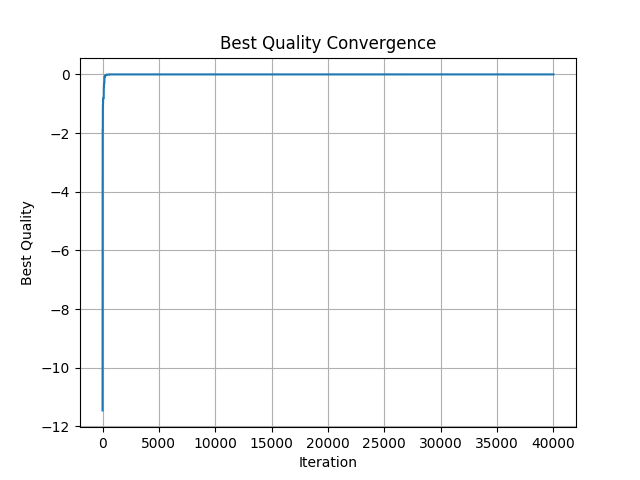
\includegraphics[width=2.8in]{./../code/test_function_result/test_best_convergence.png}
  %\vspace{-15pt}
  \caption{Test best quality convergency}
  \label{img:test_best_quality_converge}
  \end{center}
\end{figure}

\begin{figure}
  \begin{center}
  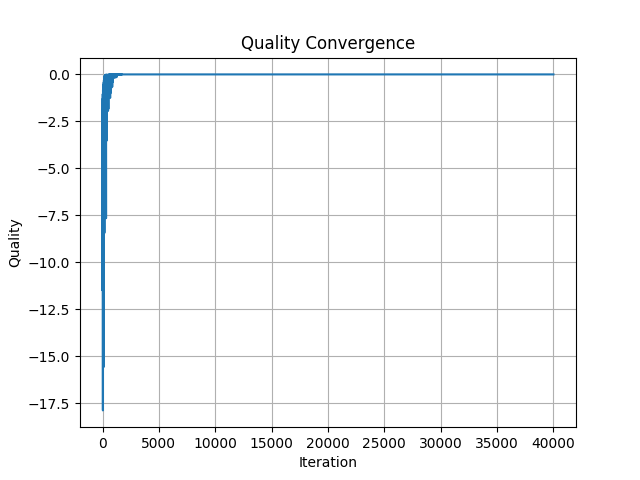
\includegraphics[width=2.8in]{./../code/test_function_result/test_quality_converge.png}
  %\vspace{-15pt}
  \caption{Test quality convergency}
  \label{img:test_quality_converge}
  \end{center}
\end{figure}

\begin{figure}
  \begin{center}
  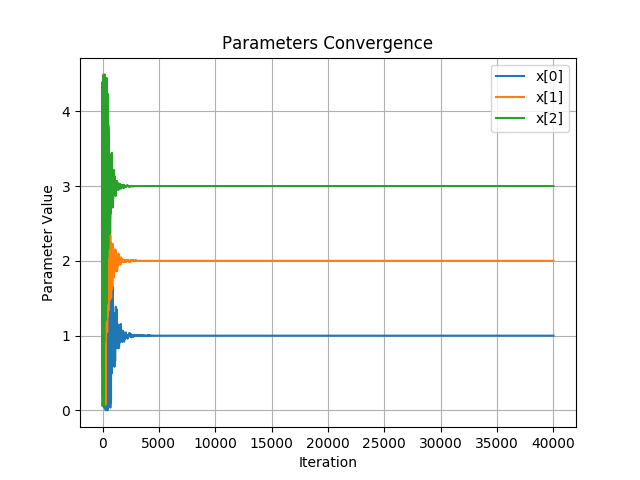
\includegraphics[width=2.8in]{./../code/test_function_result/test_parameters_converge.png}
  %\vspace{-15pt}
  \caption{Test parameters convergency}
  \label{img:test_parameters_quality_converge}
  \end{center}
\end{figure}

Thus it is clear that the algorithm works and converges accordingly. That said, the algorithm is ready to be used on the line follower problem.

\section {PSO on Line Follower Problem}

From a car circuit simulation, it was developed a line follower opmization on the \textit{proportional–integral–derivative controller (PID controller)} Control technique.

From the Equation \ref{equation:control_equation}, the objectve of this optimization is to optimize $K_p$, $K_i$, $K_d$, and the linear velocity of the car.

\begin{equation}
    \label{equation:control_equation}
    u(t) =  K_p e(t) + K_i \int_{0}^{t} e(t')dt'+K_d \frac{de(t)}{dt}
\end{equation}

In oder to do that, the \textit{PSO} algorithm was runned with 40 particles and it was developed the \textit{evaluate} method. With this method every positon of the car were evaluated and the sum of all evaluations was the score of the position of that particle.

The \textit{evaluate} method can be seen in the Code \ref{code:evaluate}, where by the end of the implementation was defined a high weight on linear speed and severe penalty for high errors and miss the track.

\lstinputlisting[
    language=python,
    caption={Method \textit{evaluate} of \textit{Simulation} Class, it is intended atribute a score for the situation of a particle.},
    label={code:evaluate},
    style=cStyle,
    firstline=130,
    lastline=152
]{./../code/simulation.py}

In the firsts tests, it was clear that the convergency was always slow and always tending first to a quite slow velocity.

Therefore a higher weight was given to linear speed and the velocity upper bounder was increased.

\subsection{Concise convercency}

After the adjustment, the algorithm was run with 40 particles for about two hours, what resulted in 5477 iterations.

The quality history and the position history can be seen in the Code \ref{code:position_pso} and Code \ref{code:quality_pso}.

The convergencies can be seen in the figures from Figure \ref{img:best_quality_converge} to Figure \ref{img:quality_converge}.

\lstinputlisting[
    language=python,
    caption={Positions results on PSO optimization, shown only the first 10 and the last 10.},
    label={code:position_pso},
    style=cStyle,
]{./../code/results/short_position_history.txt}

\lstinputlisting[
    language=python,
    caption={Quality result on PSO optimization, shown only the first 10 and the last 10},
    label={code:quality_pso},
    style=cStyle,
]{./../code/results/short_quality_history.txt}

\begin{figure}
  \begin{center}
  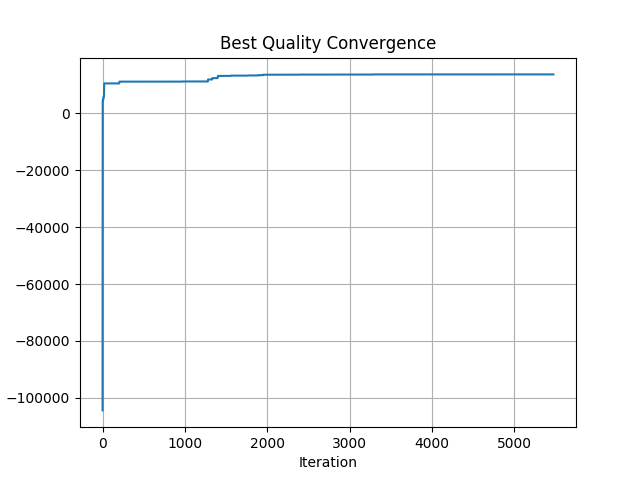
\includegraphics[width=2.8in]{./../code/results/line_best_convergence.png}
  %\vspace{-15pt}
  \caption{Best quality convergency}
  \label{img:best_quality_converge}
  \end{center}
\end{figure}

\begin{figure}
  \begin{center}
  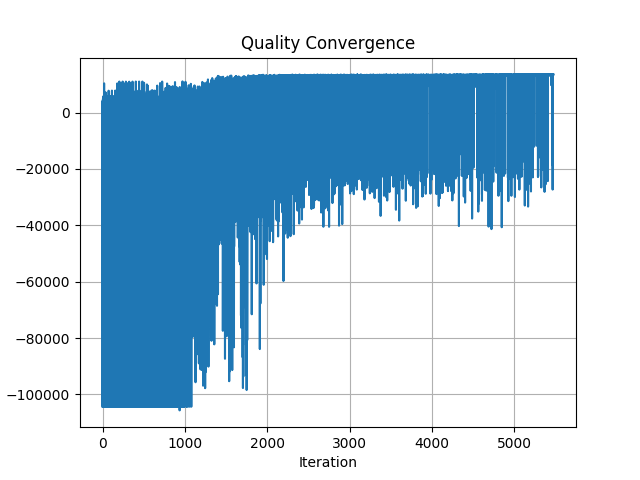
\includegraphics[width=2.8in]{./../code/results/line_quality_convergence.png}
  %\vspace{-15pt}
  \caption{Quality convergency}
  \label{img:quality_converge}
  \end{center}
\end{figure}

\begin{figure}
  \begin{center}
  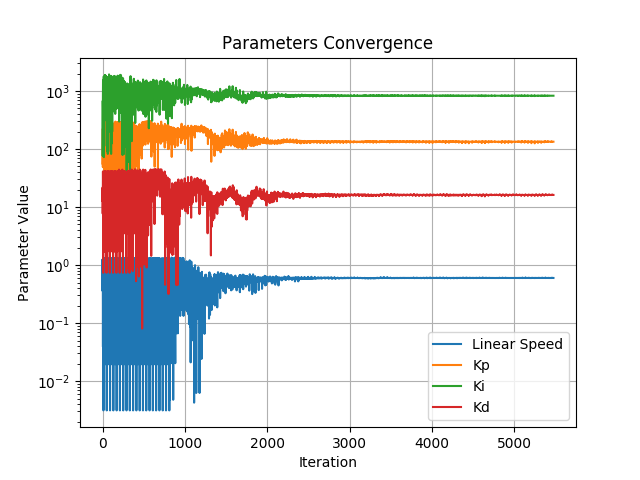
\includegraphics[width=2.8in]{./../code/results/line_parameters_convergence.png}
  %\vspace{-15pt}
  \caption{Parameters convergency}
  \label{img:parameters_quality_converge}
  \end{center}
\end{figure}

\section {Conclusion}

It was clear, therefore, that \textit{PSO} method was implemented successfully. And by analysing its results, it can be seen that \textit{PSO} has a fast conversion, but it does not converge to something necessarily great.

In fact, it finds local maximums and can easily be stocked on it. But for many cases it is good enought. In the case test, the solution found was able to complete the entire track in about 11 seconds, that is, it was realy fast and precise at the same time.

As it is possible to see on the on Figure \ref{img:initial_line_follower_solution} and Figure \ref{img:initial_line_follower_solution} that at inititals iterations the parameters are realy bad, and with the time after many itarations it has a convergency to somethig good.

\begin{figure}
  \begin{center}
  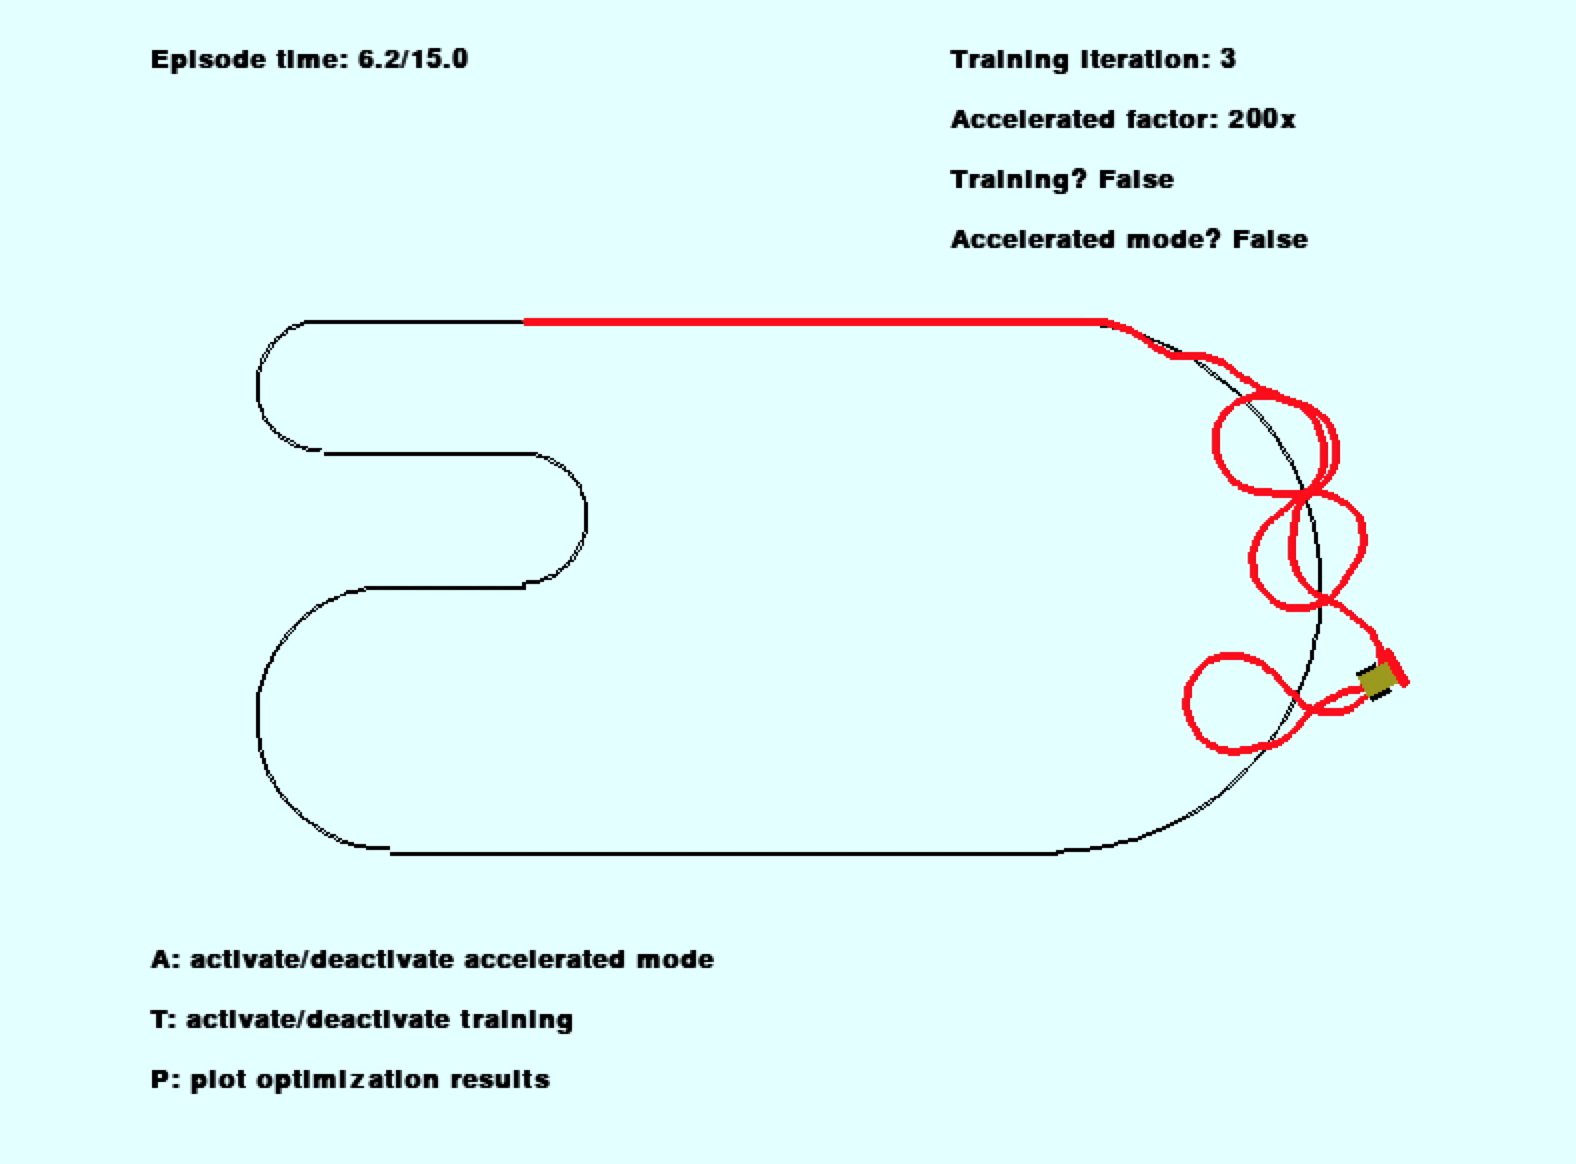
\includegraphics[width=2.8in]{./../code/results/initial_line_follower_solution.png}
  %\vspace{-15pt}
  \caption{Screenshot of the begging of the solution. Clearly the line follower was with bad parameter at this iteration.}
  \label{img:initial_line_follower_solution}
  \end{center}
\end{figure}

\begin{figure}
  \begin{center}
  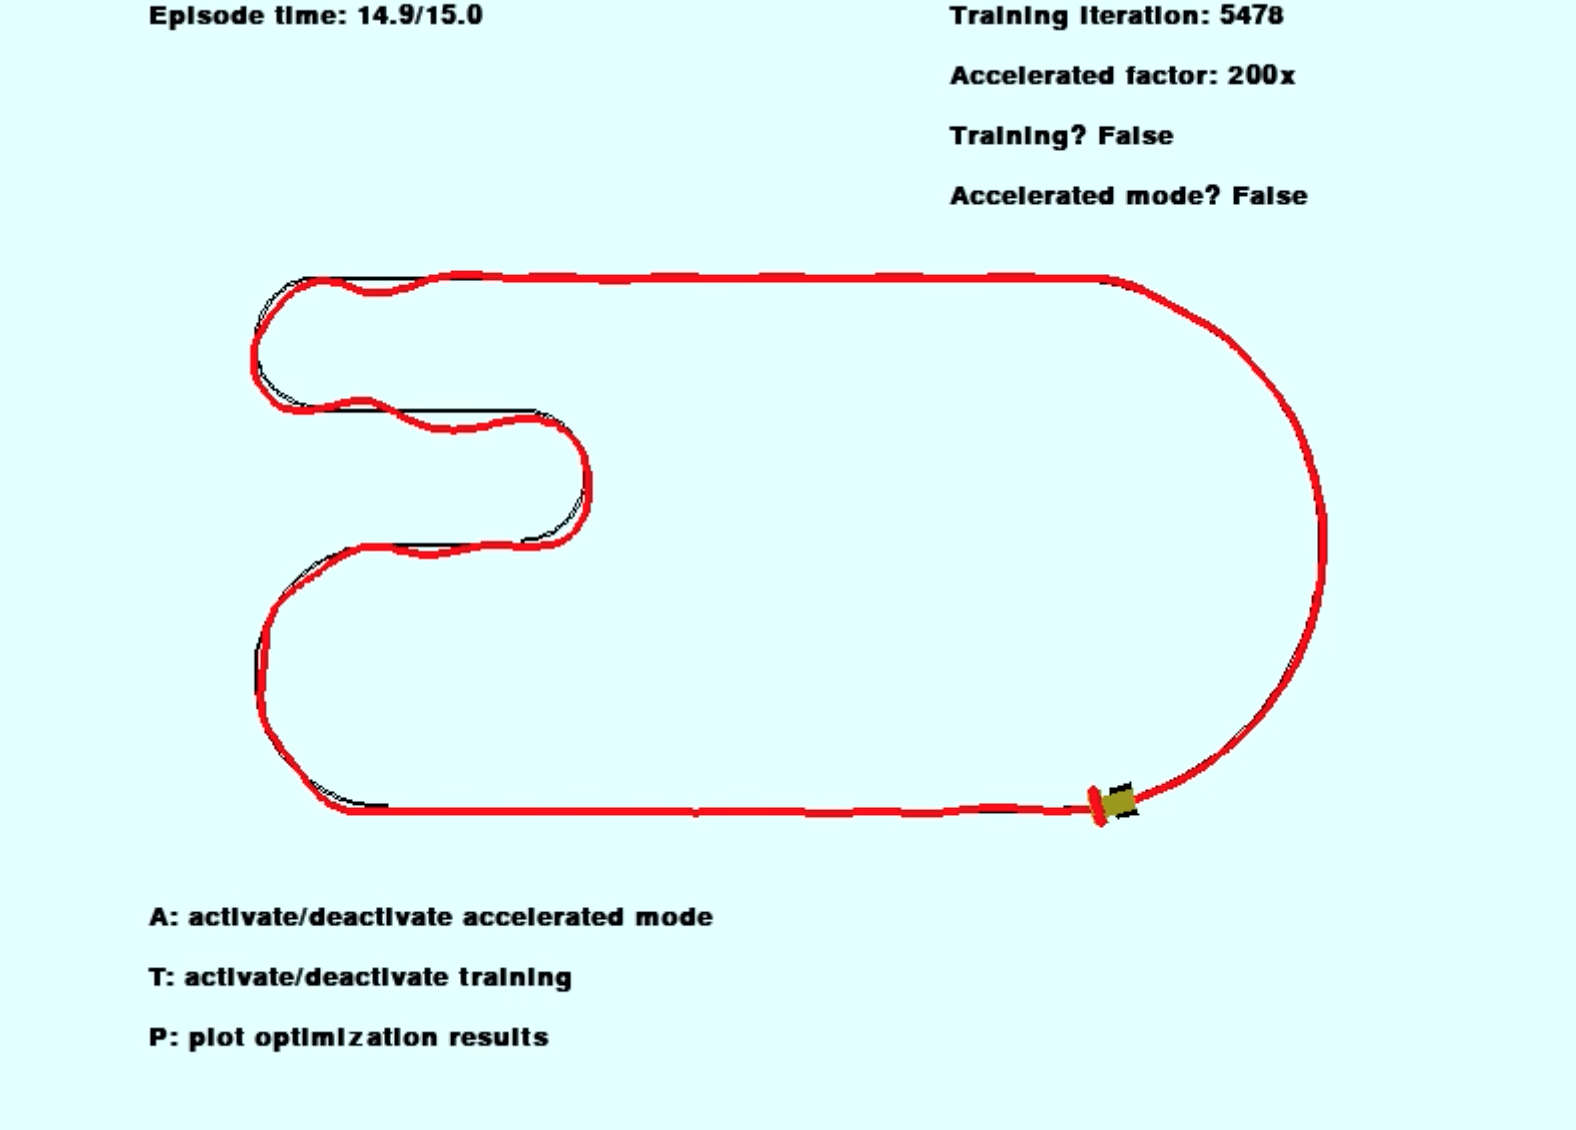
\includegraphics[width=2.8in]{./../code/results/line_follower_solution.png}
  %\vspace{-15pt}
  \caption{Screenshot at iteration number 5478. Clearly the line follower is now with good parameters.}
  \label{img:line_follower_solution}
  \end{center}
\end{figure}





\vfill
\end{document}
